% TeXworks poster recreation
% Compile with XeLaTeX in TeXworks.
%
% IMPORTANT:
% The original HTML references two external image files that were not embedded
% in the supplied HTML. Put these files in the "image" folder next to this .tex:
%   image/R-_Retraite_en_Ligne_-_Laurent_de_la_R_surrection.jpg
%   image/1.png
%
% The three embedded poster graphics and the registration-panel background
% are included with this package.

\documentclass{article}
\usepackage{geometry}
\usepackage{graphicx}
\usepackage{tikz}
\usepackage{fontspec}
\usepackage{xcolor}
\usepackage{iftex}
\pagestyle{empty}
\setlength{\parindent}{0pt}

% The InDesign export is 595.28 x 841.89 CSS pixels.
\geometry{
  paperwidth=595.28pt,
  paperheight=841.89pt,
  margin=0pt
}

% Try to use the original fonts when they are installed.
% If they are not installed, XeLaTeX falls back to close substitutes.
\IfFontExistsTF{Adobe Garamond Pro}
  {\newfontfamily\AGaramond{Adobe Garamond Pro}}
  {\newfontfamily\AGaramond{Liberation Serif}}
\IfFontExistsTF{Adobe Garamond Pro Semibold}
  {\newfontfamily\AGaramondSemi{Adobe Garamond Pro Semibold}}
  {\newfontfamily\AGaramondSemi{Liberation Serif}}
\IfFontExistsTF{DIN}
  {\newfontfamily\DINFont{DIN}}
  {\newfontfamily\DINFont{Liberation Sans}}
\IfFontExistsTF{DIN (TT) LightAlternate}
  {\newfontfamily\DINLight{DIN (TT) LightAlternate}}
  {\newfontfamily\DINLight{Liberation Sans}}
\IfFontExistsTF{DIN (TT) MediumAlternate}
  {\newfontfamily\DINMedium{DIN (TT) MediumAlternate}}
  {\newfontfamily\DINMedium{Liberation Sans}}
\IfFontExistsTF{DIN (TT) RegularAlternate}
  {\newfontfamily\DINRegular{DIN (TT) RegularAlternate}}
  {\newfontfamily\DINRegular{Liberation Sans}}
\IfFontExistsTF{DIN (TT) BoldAlternate}
  {\newfontfamily\DINBold{DIN (TT) BoldAlternate}}
  {\newfontfamily\DINBold{Liberation Sans}}

% ------------------------------------------------------------
% TRANSLATION TEXT
% Edit ONLY these definitions when making another language version.
% ------------------------------------------------------------

\newcommand{\PosterTitle}{Advent 2026 mit}
\newcommand{\OrderText}{Orden der Unbeschuhten Karmeliten}
\newcommand{\OnlineText}{Karmel Exerzitien Online}

\newcommand{\ThemeText}{«Übung der\\Gegenwart\\Gottes»}

\newcommand{\AuthorMain}{Br. Lorenz}
\newcommand{\AuthorSub}{von der Auferstehung}

\newcommand{\DateOne}{Vom 25.11.2026}
\newcommand{\DateTwo}{bis zum\\03.01.2027}

\newcommand{\Website}{online-exerzitien.karmel.at}
\newcommand{\Registration}{Anmeldung}

\newcommand{\DeliveryText}{Jeden Freitag als\\e-Mail}

\newcommand{\DescriptionText}{Eine Meditation basierend auf\\
den Texten der Heiligen Schrift\\
und des Br. Lorenz, praktische\\
Anregungen, ein Podcast der\\
Woche, der Adventskalender.}

% ------------------------------------------------------------
% Colours taken from the supplied CSS
% ------------------------------------------------------------
\definecolor{postercream}{HTML}{FCCD98}
\definecolor{posterbrown}{HTML}{4C2D1A}
\definecolor{posterwhite}{HTML}{FFFFFF}

% Position helper:
% x = distance from left edge
% y = distance from top edge
\newcommand{\PNode}[5][]{%
  \node[anchor=north west,inner sep=0pt,#1]
    at ([xshift=#2pt,yshift=-#3pt]current page.north west)
    {#4};
}

\begin{document}
\begin{tikzpicture}[remember picture,overlay]

% ------------------------------------------------------------
% IMAGE LAYERS
% These preserve the original InDesign container coordinates.
% ------------------------------------------------------------

% Main photograph/background: _idContainer000
\IfFileExists{image/R-_Retraite_en_Ligne_-_Laurent_de_la_R_surrection.jpg}{%
  \node[anchor=north west,inner sep=0pt]
    at ([xshift=-28.347pt,yshift=23.386pt]current page.north west)
    {
\includegraphics[width=638.36pt,height=836.22pt]{image/R-_Retraite_en_Ligne_-_Laurent_de_la_R_surrection.jpg}};
}{%
  % Visible compile-time placeholder if the source photo has not been copied.
  \node[anchor=north west,inner sep=0pt]
    at ([xshift=0pt,yshift=0pt]current page.north west)
    {\parbox[c][841.89pt][c]{595.28pt}{\centering\Large
      Missing background image:\\
      \texttt{R-\_Retraite\_en\_Ligne\_-...jpg}}};
}

% _idContainer001 — original external image 1.png
\IfFileExists{image/1.png}{%
  \node[anchor=north west,inner sep=0pt]
    at ([xshift=-62.300pt,yshift=-796.450pt]current page.north west)
    {
\includegraphics[width=688.69pt,height=54.63pt]{image/1.png}};
}{}

% _idContainer003 — embedded small emblem
\node[anchor=north west,inner sep=0pt]
  at ([xshift=7.086pt,yshift=-788.829pt]current page.north west)
  {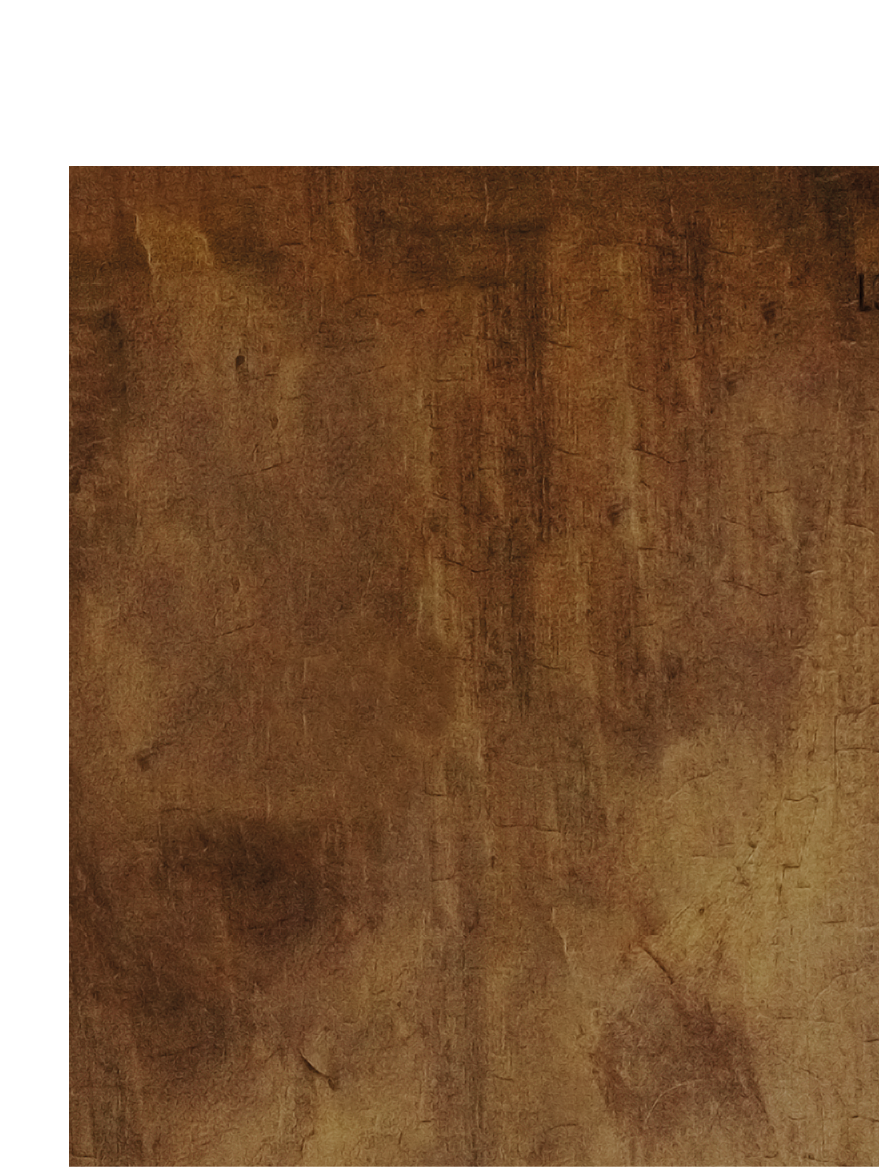
\includegraphics[width=32.53pt,height=50.93pt]{R-_Retraite_en_Ligne_-_Laurent_de_la_R_surrection_v2_verso.png}};

% _idContainer009 — embedded lower graphic
\node[anchor=north west,inner sep=0pt]
  at ([xshift=118.172pt,yshift=-698.033pt]current page.north west)
  {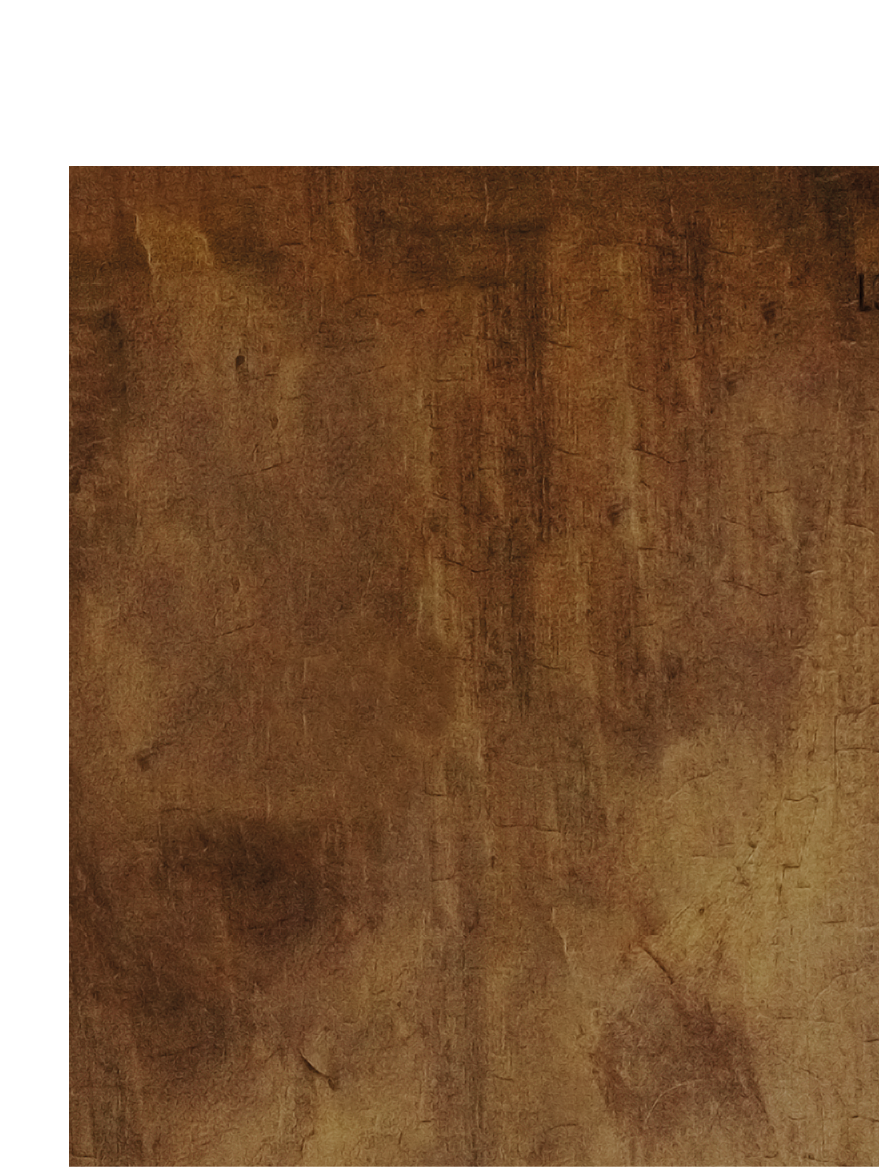
\includegraphics[width=467.26pt,height=98.44pt]{R-_Retraite_en_Ligne_-_Laurent_de_la_R_surrection_v2_verso.png}};

% _idContainer010 — registration panel background
\node[anchor=north west,inner sep=0pt]
  at ([xshift=120.476pt,yshift=-729.565pt]current page.north west)
  {
\includegraphics[width=415.34pt,height=75.09pt]{poster_button_bg.png}};

% _idContainer014 — embedded small emblem
\node[anchor=north west,inner sep=0pt]
  at ([xshift=525.749pt,yshift=-719.230pt]current page.north west)
  {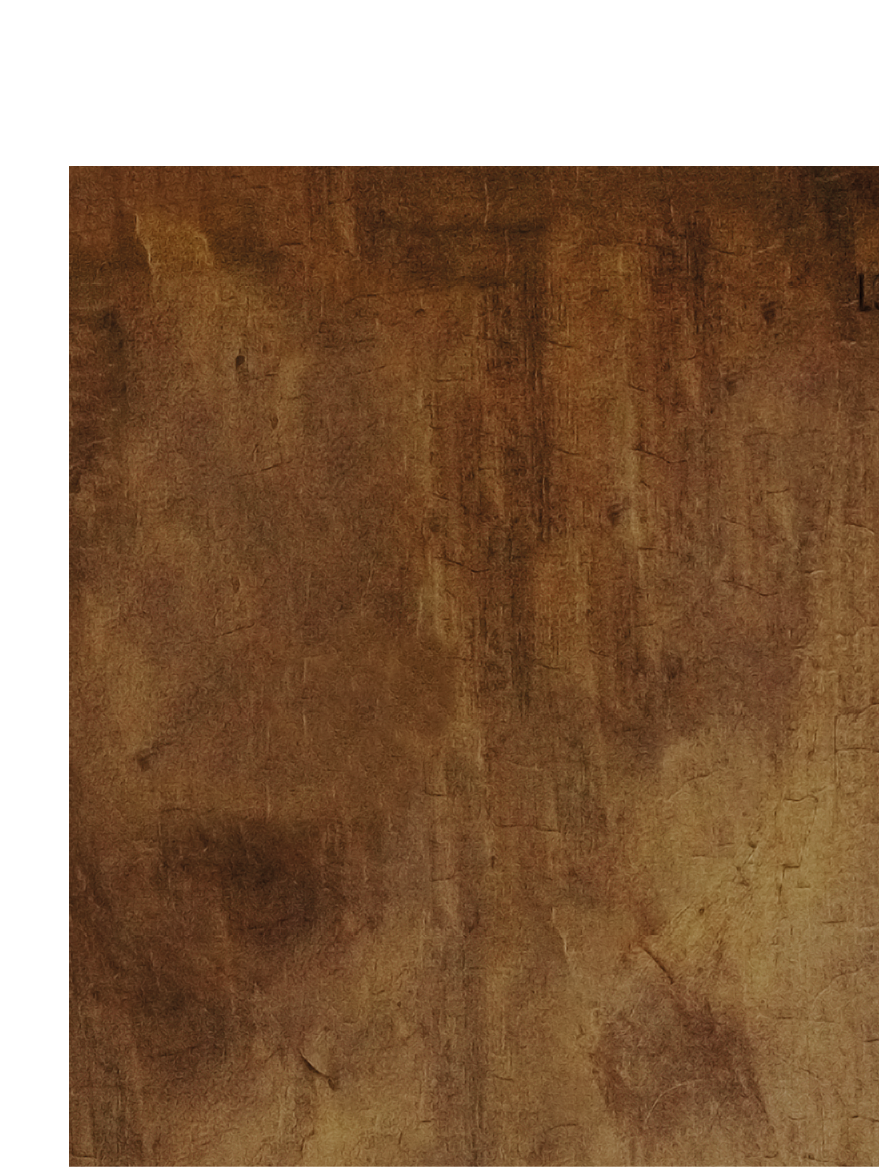
\includegraphics[width=45.15pt,height=57.77pt]{R-_Retraite_en_Ligne_-_Laurent_de_la_R_surrection_v2_verso.png}};

% ------------------------------------------------------------
% TEXT LAYERS
% Coordinates are converted from the original CSS + scale(0.05).
% ------------------------------------------------------------

% Advent 2026 mit
\PNode[font=\AGaramond\fontsize{30.8pt}{30.8pt}\selectfont\scshape,
       text=posterwhite]
      {242.435}{82.199}{\PosterTitle}

% Orden der Unbeschuhten Karmeliten
\PNode[font=\AGaramond\fontsize{42pt}{42pt}\selectfont\scshape,
       text=posterwhite]
      {44.819}{815.672}{\OrderText}

% Karmel Exerzitien Online
\PNode[font=\DINMedium\fontsize{42pt}{42pt}\selectfont\scshape,
       text=posterwhite]
      {-0.001}{24.795}{\OnlineText}

% «Übung der Gegenwart Gottes»
\PNode[font=\AGaramond\fontsize{41.9pt}{41.9pt}\selectfont,
       text=posterwhite]
      {332.707}{246.687}{\ThemeText}

% Br. Lorenz
\PNode[font=\AGaramond\fontsize{67pt}{67pt}\selectfont\scshape,
       text=posterwhite]
      {246.685}{123.641}{\AuthorMain}

% von der Auferstehung
\PNode[font=\AGaramond\fontsize{32pt}{32pt}\selectfont\scshape,
       text=posterwhite]
      {246.685}{187.016}{\AuthorSub}

% Dates
\PNode[font=\DINLight\fontsize{30.8pt}{30.8pt}\selectfont\scshape,
       text=posterwhite]
      {367.995}{385.800}{\DateOne}

\PNode[font=\DINLight\fontsize{30.8pt}{30.8pt}\selectfont\scshape,
       text=posterwhite]
      {359.195}{421.000}{\DateTwo}

% Website
\PNode[font=\DINBold\fontsize{26.5pt}{26.5pt}\selectfont,
       text=postercream]
      {180.635}{754.248}{\Website}

% Registration
\PNode[font=\DINRegular\fontsize{30.8pt}{30.8pt}\selectfont\scshape,
       text=postercream]
      {255.447}{716.718}{\Registration}

% Delivery
\PNode[font=\DINRegular\fontsize{17pt}{17pt}\selectfont\scshape,
       text=posterwhite]
      {390.744}{505.897}{\DeliveryText}

% Description
\PNode[font=\DINFont\fontsize{14pt}{14pt}\selectfont,
       text=posterwhite]
      {390.551}{545.424}{\DescriptionText}

\end{tikzpicture}
\end{document}
